\documentclass{article}
\usepackage{graphicx} % new way of doing eps files
\usepackage{listings} % nice code layout
\usepackage[usenames]{color} % color
\usepackage{float}
\definecolor{listinggray}{gray}{0.9}
\definecolor{graphgray}{gray}{0.7}
\definecolor{ans}{rgb}{1,0,0}
\definecolor{blue}{rgb}{0,0,1}
% \Verilog{title}{label}{file}
\newcommand{\Verilog}[3]{
  \lstset{language=Verilog}
  \lstset{backgroundcolor=\color{listinggray},rulecolor=\color{blue}}
  \lstset{linewidth=\textwidth}
  \lstset{commentstyle=\textit, stringstyle=\upshape,showspaces=false}
  \lstset{frame=tb}
  \lstinputlisting[caption={#1},label={#2}]{#3}
}


\author{Jiasen Zhou, Jon Johnston}
\title{Lab 11}

\begin{document}
\maketitle

\section{Executive Summary}
This lab had three parts: creating the Write Back stage, integrating it into the datapath, and then testing the datapath with code that performs a simple division. For the Write Back stage, a new module did not have to be created, a mux was simply added to the current datapath. However, an iWriteBack module was created to nest the mux for ease of reading. The division test did not require a new module to be created either, machine code for the division simply had to be created and implemented in the instruction memory file. The reg data and memory files also had to be edited to ensure correct operation. The division of 21 by 7 correctly produced the result of 3, demonstrating that all three parts of the lab were successful.

\section{Test Report}
To verify operation of these modules, this lab required two test benches. 
\begin{enumerate}
	\item Datapath Test Bench
	\item Division Test Bench
\end{enumerate}

\subsection{Datapath Test Bench}
The Datapath Test Bench contains:
\begin{enumerate}
	\item Inputs
	\begin{enumerate}
		\item reset - reset button that sets PC source to 0
	\end{enumerate}	
	\item Outputs
	\begin{enumerate}	
		\item read\_data1 - data stored in read register 1
		\item read\_data2 - data stored in read register 2
		\item write\_data - the output of the Write Back stage 
	\end{enumerate}
\end{enumerate} 

\subsection{Division Test Bench}
The Divison Test Bench contains:
\begin{enumerate}
	\item Inputs
	\begin{enumerate}
		\item reset - reset button that sets PC source to 0
	\end{enumerate}	
	\item Outputs
	\begin{enumerate}	
		\item read\_data1 - data stored in read register 1
		\item read\_data2 - data stored in read register 2
		\item write\_data - the output of the Write Back stage 
	\end{enumerate}
\end{enumerate} 

\pagebreak

\begin{figure}
	\begin{center}
		\caption{Expected Results of the Datapath test.}\label{fig:ert_registertest}
		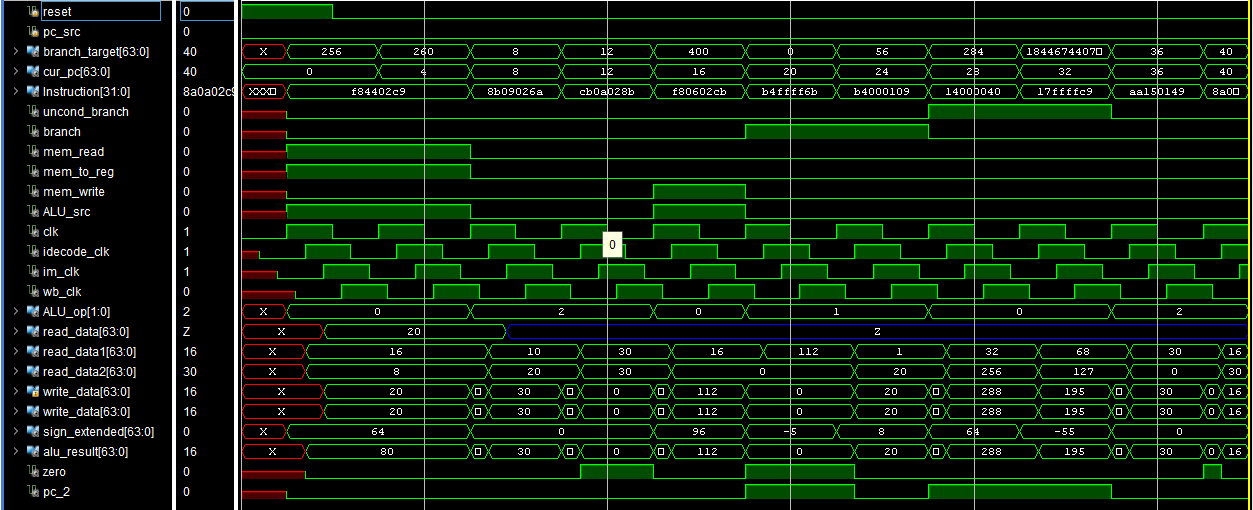
\includegraphics[width=1.0\textwidth]{../images/Lab11_datapath_timing_diagram.png}
	\end{center}
\end{figure}

\begin{figure}
	\begin{center}
		\caption{Timing diagram for the Division test.}\label{fig:registertest}
		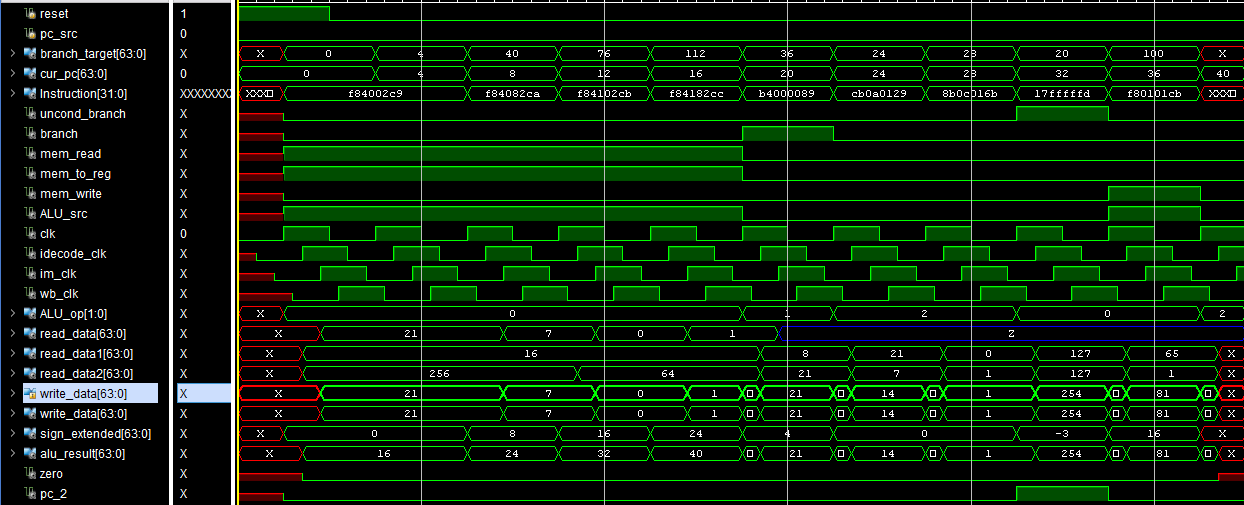
\includegraphics[width=1.0\textwidth]{../images/Lab11_division_timing_diagram.png}
	\end{center}
\end{figure}




\section{Code Appendix}
% The code appendix should include the test bench code and module code for this lab.
\Verilog{Verilog code for testing a register.}{code:regtest}{../code/2_decode/datapath.v}

\end{document} 